\newpage
\section{Praktikum 4 - Teil I: Topic Modell Parameter und Interpretation (Common-Crawl)}

\subsection{Topic Überbegriffe}


\includegraphics[width=0.5\textwidth]{images/cc0.png}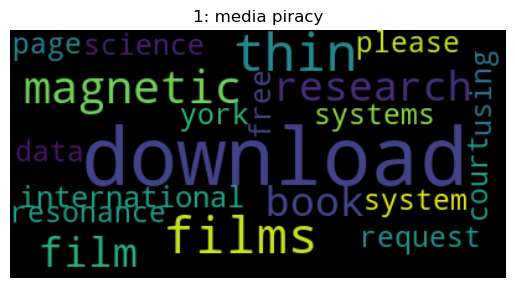
\includegraphics[width=0.5\textwidth]{images/cc1.png} \\
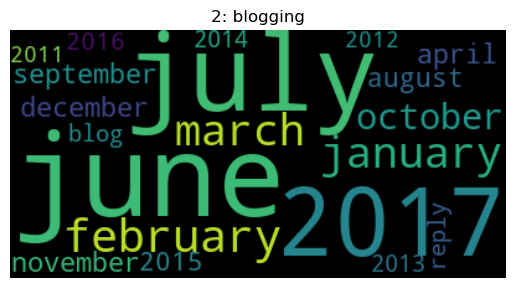
\includegraphics[width=0.5\textwidth]{images/cc2.png}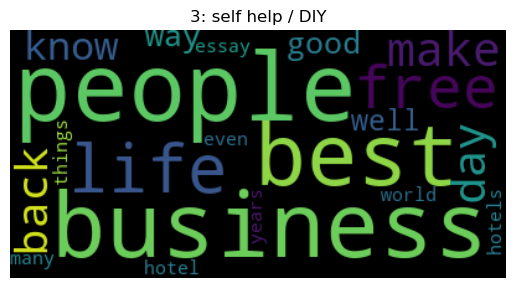
\includegraphics[width=0.5\textwidth]{images/cc3.png} \\
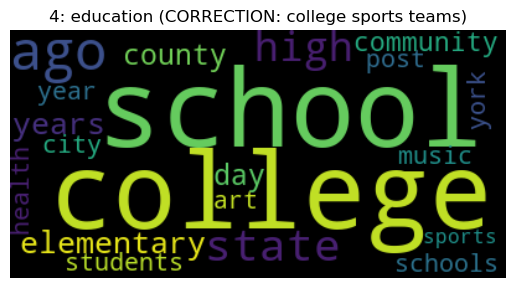
\includegraphics[width=0.5\textwidth]{images/cc4.png}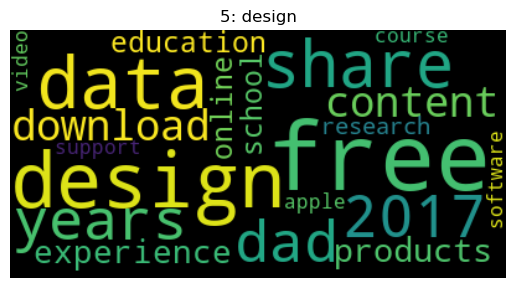
\includegraphics[width=0.5\textwidth]{images/cc5.png} \\
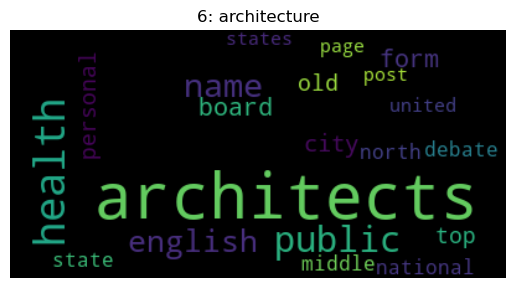
\includegraphics[width=0.5\textwidth]{images/cc6.png}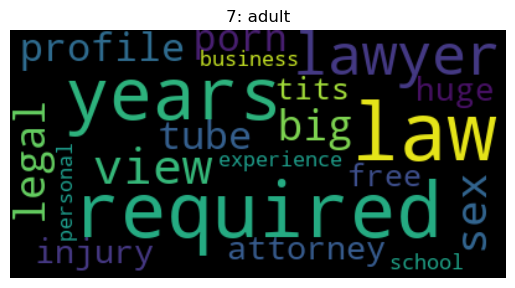
\includegraphics[width=0.5\textwidth]{images/cc7.png} \\
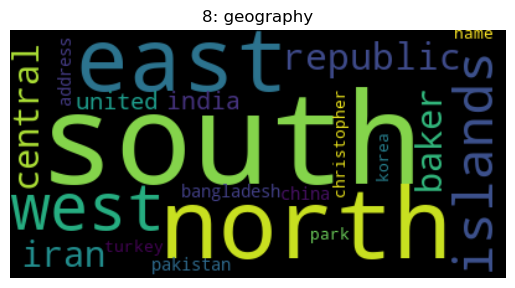
\includegraphics[width=0.5\textwidth]{images/cc8.png}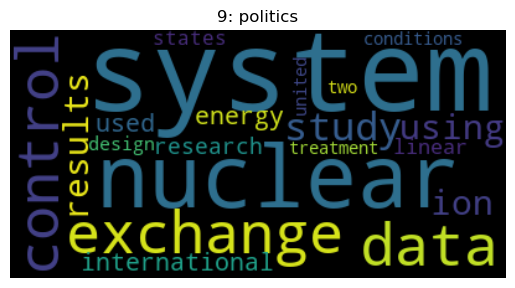
\includegraphics[width=0.5\textwidth]{images/cc9.png} \\
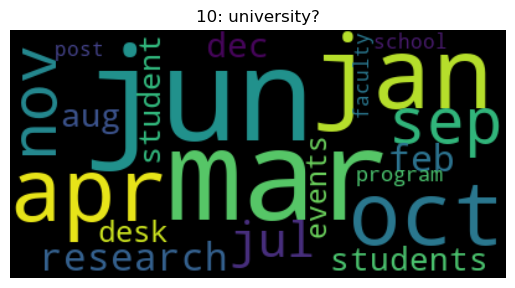
\includegraphics[width=0.5\textwidth]{images/cc10.png}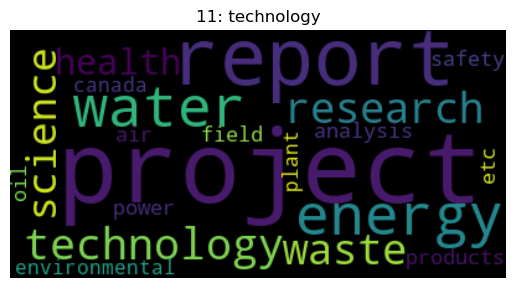
\includegraphics[width=0.5\textwidth]{images/cc11.png} \\
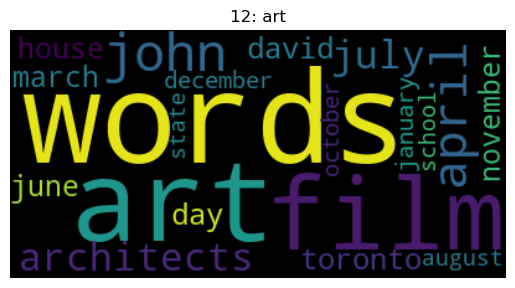
\includegraphics[width=0.5\textwidth]{images/cc12.png}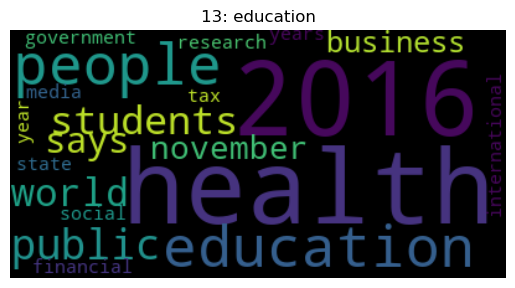
\includegraphics[width=0.5\textwidth]{images/cc13.png} \\
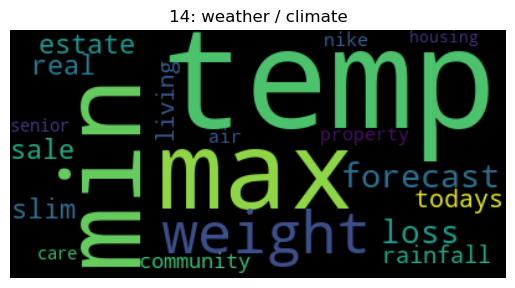
\includegraphics[width=0.5\textwidth]{images/cc14.png} \\

\noindent Mit Ausnahme von 10: University erscheinen alle relativ sinnvoll, unter Berücksichtigung dass sich die Qualität der Topics unterscheidet

\subsection{Filter Adult Topic}

{\color{MidnightBlue}
\begin{lstlisting}[language=python]
censored_result = result[(dfnormal[7] <= 0.5) | (dfnormal[7].isna())]
censored_dfnormal = dfnormal[(dfnormal[7] <= 0.5) | (dfnormal[7].isna())]
\end{lstlisting}}

\noindent Wir entfernen hier aus dem CC Datensatz alle Dokumente mit einer Wahrscheinlichkeit über 50\% des Adult Topics (7).

\subsection{Stichproben}

Education Topic (4) mit über 70\% Wahrscheinlichkeit: \\

{\color{MidnightBlue}
\noindent\url{http://lmmc.ca/en/concert_details.php?concert_id=114} \\
\url{https://www.620ckrm.com/2017/03/11/regina-cougars-wbb-team-to-play-in-usports-canada-consolation-final/} \\
\url{http://feathermerchant.com/?category=sports%3Ecollege&id=363&type=golf%20towel} \\
\url{https://www.thestudentroom.co.uk/showthread.php?t=5012052} \\
\url{http://ginasbluewaterbabies.com.au/category/uncategorized/page/2/} \\
\url{http://gamestrailer.info/universities-in-newcastle-upon-tyne/} \\
\url{https://www.delgazette.com/wire/state-wire/55244/ohio-student-athlete-badly-hurt-in-makeshift-pool-at-party} \\
\url{http://osuvetjobs.org/jobs/10946747/experienced-vet-tech-needed-in-busy-4-doctor-practice} \\
\url{https://www.roero-illuminazione.it/cms/community/social/immagini/foto-community.html} \\
\url{http://www.kofc.org/en/columbia/detail/2012_08_legacy.html}} \\

\noindent Wir würden hier den Topic Überbegriff von Education Topic (4) auf College Sports Teams Topic (4) korrigieren. Wir haben uns auch einige andere angeschaut, mussten aber sonst keine Korrigierungen vornehmen.

\subsection{Topic Mischungen}

Blogging Topic (2) und College Sports Teams Topic (4) zu jeweils mindestens 40\%: \\

{\color{MidnightBlue}
\noindent\url{https://nevadacycling.wordpress.com/2012/09/} \\
\url{https://navarrepress.com/tag/races/} \\
\url{http://thepipelineshow.blogspot.com/2012/04/whl-dominates-chl-attendance-numbers.html} \\
\url{http://southfloridasport.blogspot.com/2016/02/miami-ratings-january-2016.html} \\
\url{https://postinspostcards.com/2015/12/02/cfa-2015-game-103-cincinnati-at-usf-nov-20/} \\
\url{http://photos.gardner-webb.edu/2016-Photos/December-2016/Shanghai-Faculty-Visit/i-gKr3BXd/} \\
\url{http://unitykhartoum.blogspot.com/2014/09/an-exchange-of-emails-between-dr-marina.html} \\
\url{https://buifc.wordpress.com/upcoming-events/} \\
\url{http://eagles-rju.blogspot.com/2018/06/four-ncaa-skaters-among-first-14-taken.html} \\
\url{http://eagles-rju.blogspot.com/2015/09/}} \\

\noindent Die erhaltenen Dokumente sind Sports Blogs, somit exakt was wir gesucht haben.

\subsection{Zwei neue Modelle}

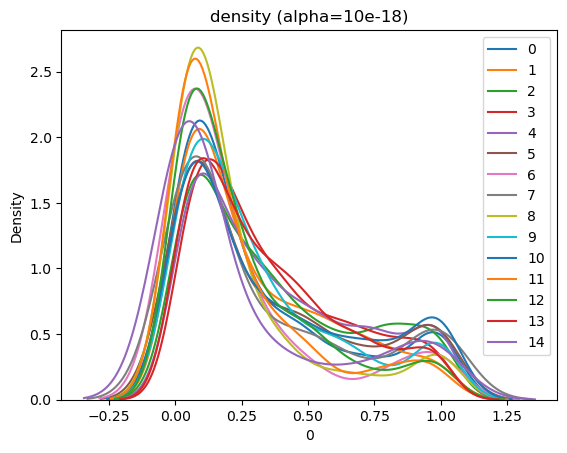
\includegraphics[width=0.33\textwidth]{images/alpha=10e-18.png}
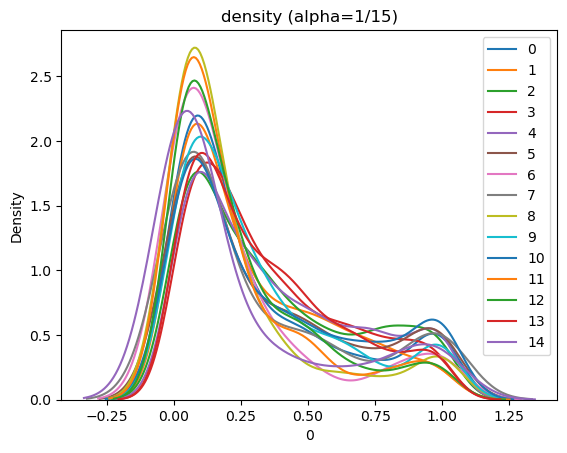
\includegraphics[width=0.33\textwidth]{images/alpha=0.066.png}
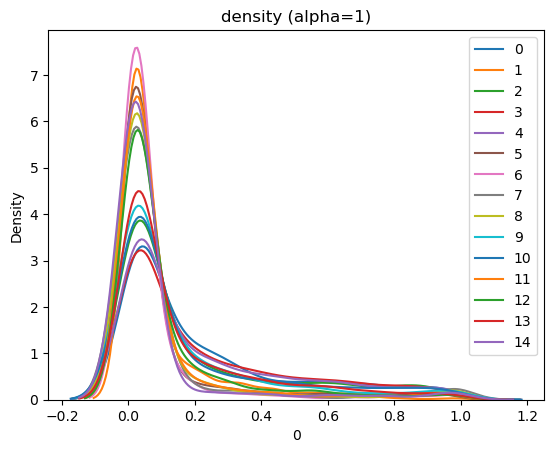
\includegraphics[width=0.33\textwidth]{images/alpha=1.png}

\noindent Geplottet sind hier für die drei Modelle je Topic die Häufigkeiten für Wahrscheinlichkeitswerte im Corpus. Wie man sieht verschwindet mit zunehmendem Glättungsparameter der zweite Höhepunkt um die 1. Das liegt daran, dass pro Dokument die Topicwahrscheinlichkeiten geglättet werden, das Modell somit weniger annimmt, dass dem Dokument nur ein Topic unterliegt.

\setcounter{section}{3}
\section{Praktikum 4 - Teil II: Topic Modell auf eigenen gecrawlten Texten}

\subsection{Topic Überbegriffe}

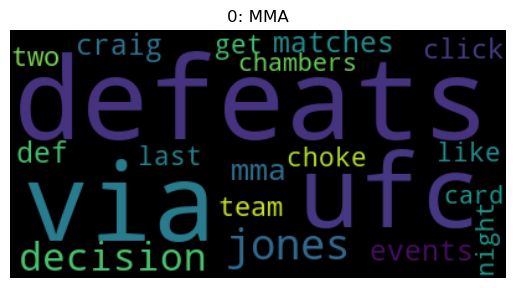
\includegraphics[width=0.5\textwidth]{images/gi0.png}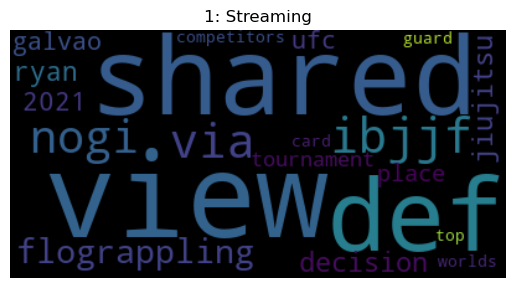
\includegraphics[width=0.5\textwidth]{images/gi1.png} \\
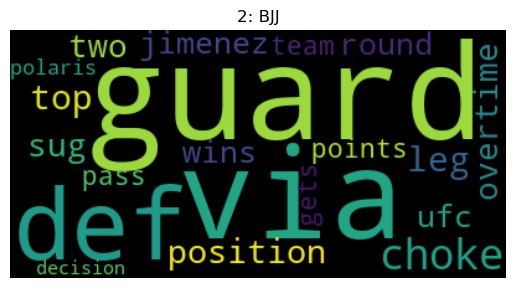
\includegraphics[width=0.5\textwidth]{images/gi2.png}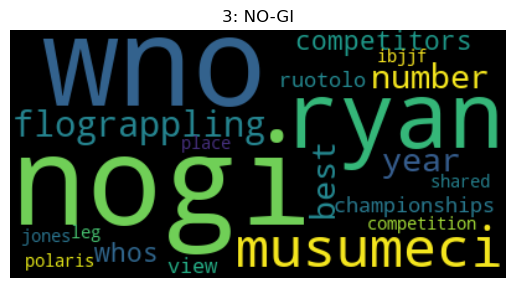
\includegraphics[width=0.5\textwidth]{images/gi3.png} \\
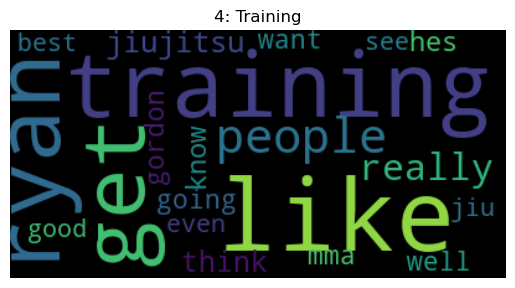
\includegraphics[width=0.5\textwidth]{images/gi4.png}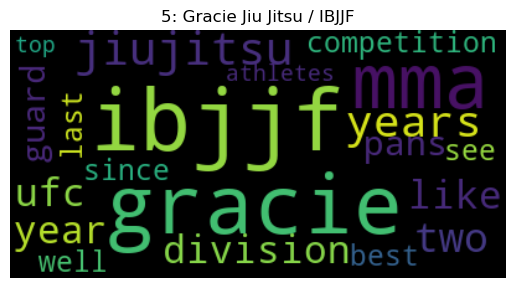
\includegraphics[width=0.5\textwidth]{images/gi5.png} \\

\noindent Erscheinen alle sinnvoll, wobei wir hier auch eine Topicanzahl gewählt haben über die es hinaus weniger sinnvoll wurde.

\subsection{Filter Adult Topic}

Unser Datensatz beinhaltet keinen Adult Content.

\subsection{Stichproben}

Da wir in unserem Datensatz die Titel haben, haben wir diese statt den Links ausgegeben:

{\color{MidnightBlue}
\begin{lstlisting}
0 MMA
Video: On closer look, Aljamain Sterling appears to tap to Damien Nitkin at High..
Who's Next episode 6 results and recap: The final is set
'Ready to get famous?': Who’s Next episode 1 recap and results
Mike Tyson, Wiz Khalifa, and Nate Diaz sponsor athletes at High Rollerz 15
FloGrappling's Who’s Next: Submission Fighter Challenge reality show set for May..
Chael Sonnen Hints That Submission Underground Will Move to FloGrappling
Craig Jones Vs. UFC's Donald 'Cowboy' Cerrone In Combat Jiu-Jitsu Worlds 2021
Dillon Danis Ejected From UFC 268, Slapped by Manager Ali Abdelaziz
High Rollerz: Cops Vs Stonerz – 18 September!
Demian Maia Not Ready to Retire Yet, Plans to Compete in Jiu-Jitsu
\end{lstlisting}}

\noindent$\Rightarrow$ Passt in etwa, aber sehr hit and miss.

{\color{MidnightBlue}
\begin{lstlisting}
1 Streaming
Gordon Ryan insists on no-time-limit stipulation in fourth Felipe Pena match
2022 IBJJF no-gi Pans recap and black belt results
Weekend grappling recap: Polaris 21 and IBJJF Atlanta Open results
Renato Canuto vs. Tommy Langaker booked for ONE 160
WNO: Gordon Ryan vs. Felipe Pena full event results and video highlights
FloGrappling releases statement about Ryan vs. Pena match controversy
Sub Only Series VII results and highlights: PJ Barch submits four in a row
Josh Cisneros vs. Damien Anderson booked for Fight To Win title
WNO: Gordon Ryan vs. Felipe Pena full card line-up and preview
Dates and location set for 2022 IBJJF no-gi Worlds
\end{lstlisting}}

\noindent$\Rightarrow$ Passt in etwa auf Event Streaming.

{\color{MidnightBlue}
\begin{lstlisting}
2 BJJ
Polaris 20: USA Vs Brazil Results
UFC 274: Oliveira Submits Gaethje with RNC
Polaris 19 results and highlights: Roberto Jimenez dominates, Ash Williams and..
Emerald City Invitational results and highlights: Underdog Kieran Kichuk wins $10K
SUG 29 Results: Andy Varela Taps Sean Strickland in Bizarre Main Event
Polaris 18 Results and Video Highlights: Ashley Williams Upsets Paulo Miyao
Raw Grappling 1 Results and Highlights: Yuri Simoes Wins 8-Man Grand Prix
SUG 28 Results and Highlights: Andy Varela Upsets Haisam Rida in Main Event
Polaris 17 Results and Highlights: Craig Jones Retains Title Against Cautious Davi..
SUG 27 Results and Video Highlights: Mason Fowler Retains Title Against Gabriel..
\end{lstlisting}}

\noindent$\Rightarrow$ Sollte eher Ergebnisse und Highlights hei{\ss}en.

{\color{MidnightBlue}
\begin{lstlisting}
3 NO-GI
Mikey Musumeci beats Cleber Sousa to capture first-ever ONE submission grappling..
Nick Rodriguez, Giancarlo Bodoni and others set for a stacked EBI 20
Match preview: Mikey Musumeci vs. Cleber Sousa for first-ever ONE submission..
Full main card revealed for WNO: Pedro Marinho vs. Giancarlo Bodoni
Mikey Musumeci vs. Cleber Sousa booked for first ever ONE submission grappling..
Gordon Ryan Vs Felipe Pena: WNO Announce Major Line Up
Jacob Couch vs. Eoghan O'Flanagan set for Grapplefest championship
Giancarlo Bodoni replaces Andy Varela to face Jacob Rodriguez at Who's Number One
Jessa Khan to make ONE Championship debut against Amanda 'Tubby' Alequin
Tim Spriggs stripped of WNO title, Gordon Ryan vs. Pedro Marinho now for..
\end{lstlisting}}

\noindent$\Rightarrow$ Passt sehr gut.

{\color{MidnightBlue}
\begin{lstlisting}
4 Training
Like mother, like son: How Rodrigo Marello's mom taught him jiu-jitsu and more
John Danaher Promotes Nathalia Santoro to BJJ Brown Belt
Competition Tips for BJJ Beginners with Emily Eyles
John Danaher, Craig Jones talk about conflict behind DDS split
Kade Ruotolo: 'If I were to roll with Gordon, I don't think he can heel hook me'
ADCC interview: Ash Williams is ready to make history
Mark Zuckerberg Trains Brazilian Jiu-Jitsu
'Buchecha' is confident ONE Championship title shot will 'happen naturally'
Matty Healy Spotted Doing Brazilian Jiu-Jitsu
'I'm on a new level': Renato Canuto is ready for ONE Championship debut against..
\end{lstlisting}}

\noindent$\Rightarrow$ Passt sehr gut.

{\color{MidnightBlue}
\begin{lstlisting}
5 Gracie Jiu Jitsu / IBJJF
UFC Champ Leon Edwards Awarded BJJ Black Belt
Mikey Musumeci wants grappling match against Demetrious Johnson
Video: Watch Rodrigo Marello's record-setting $50,000 foot lock
Dave Mustaine Promoted to BJJ Brown Belt
Roger Gracie Gets Promoted to 5th Degree Black Belt
Leandro Lo killed in nightclub shooting
Abraham Lincoln: Hall of Fame Wrestler
Ffion Davies becomes the first Brit to ever make black belt final at IBJJF Worlds
Owen Livesey Promoted to BJJ Black Belt
Checkmat's Elder Cruz promoted to black belt
\end{lstlisting}}

\noindent$\Rightarrow$ Sollte eher Promotionen und Kontroversen hei{\ss}en.

\subsection{Topic Mischungen}

Results \& Highlights Topic (2) und NO-GI Topic (3) zu jeweils mindestens 40\%: \\

{\color{MidnightBlue}
\begin{lstlisting}
Video: Ashley Williams Submits Robert Degle at Grapple Kings 6                  
Beyond The Match: Re-live Andrew Wiltse's Comeback Submission on Gabriel Almeida
JT Torres, Edwin Najmi to Represent Team USA at Polaris Squads                  
Polaris Squads to Return With Team USA vs. Team UK and Ireland                  
Polaris 12: The Undercard's Hidden Gems                                         
ADCC 2019 Results: Craig Jones Chokes Out Thor                                  
ADCC 2019 Results: Craig Jones vs Ben Dyson                                     
Ross Nicholls vs. Vagner Rocha set for Polaris 9
\end{lstlisting}}

\noindent Die erhaltenen Dokumente sind Ergebnisse und Highlights zu No-Gi Wettkämpfen, somit exakt was wir gesucht haben.

\subsection{Zwei neue Modelle}

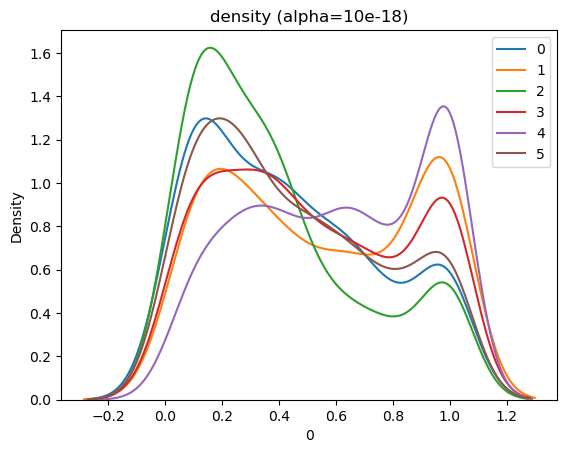
\includegraphics[width=0.33\textwidth]{images/grappling_alpha=10e-18.png}
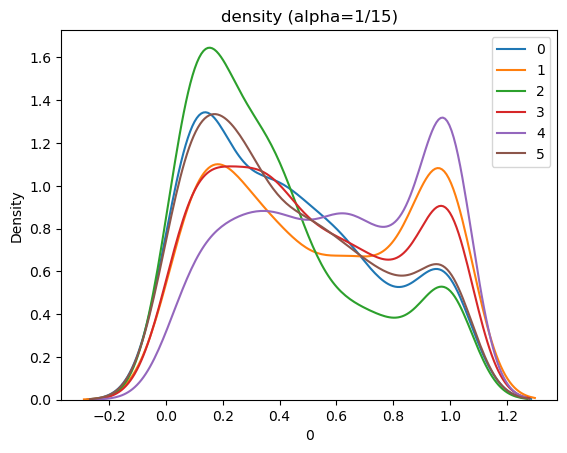
\includegraphics[width=0.33\textwidth]{images/grappling_alpha=0.066.png}
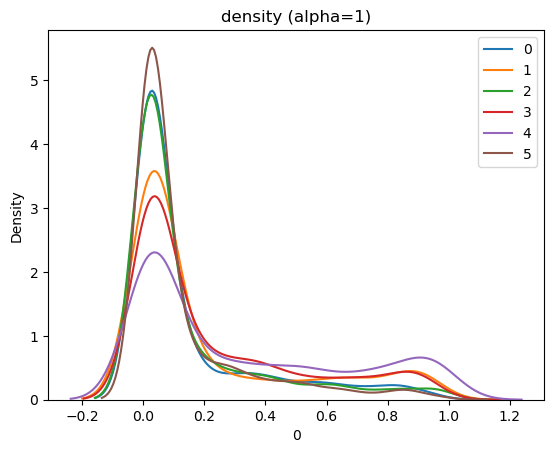
\includegraphics[width=0.33\textwidth]{images/grappling_alpha=1.png}

\noindent Geplottet sind auch hier wieder für die drei Modelle je Topic die Häufigkeiten für Wahrscheinlichkeitswerte im Corpus. Man beobachtet wieder ein mit zunehmendem Glättungsparameter verschwindender zweite Höhepunkt um die 1 aufgrund dessen, dass pro Dokument die Topicwahrscheinlichkeiten geglättet werden und das Modell somit weniger annimmt, dass dem Dokument nur ein Topic unterliegt.